\section{Agentic Engineering}
We describe the transition from \textbf{vibe coding} (human prompting) to \textbf{agentic engineering}.
In vibe coding, a human prompts an AI model to write code. In agentic engineering, AI agents write the code themselves. They plan, implement, and iterate. 
To support these long-horizon tasks, GLM-5 utilizes a fully asynchronous and decoupled RL framework to significantly boost GPU utilization by reducing idle time during agent rollouts. 
To scaling agent environments, we have developed environment-building pipelines. For coding tasks, we set up real-world  software engineering issues and terminal tasks by creating over 10,000 verifiable training scenarios. For search agents, we develop an automatic and scalable complex multi-step reasoning data synthesis pipeline to build data for agentic training.


\subsection{Asynchronous RL for Agentic Tasks}
To conduct RL for agent tasks, we design a fully asynchronous and decoupled RL infrastructure that efficiently handles long-horizon agent rollouts and supports flexible multi-task RL training across diverse agent frameworks.


We adopt the group-wise policy optimization algorithm for RL training.
For each problem \(x\), we sample \(K\) agent traces \(\{y_1,\dots,y_K\}\) from the previous policy
\(\pi_{\text{old}}\), and optimize the model \(\pi_\theta\) with respect to the following objective:
\[
L(\theta)
   = \mathbb{E}_{x\sim\mathcal{D}}\!\left[
        \frac{1}{K}\sum_{i=1}^{K}
        \left(
            r(x,y_i) - \bar{r}(x)
        \right)
     \right],
\]
where $\bar{r}(x) \;=\; \frac{1}{K}\sum_{i=1}^{K} r\bigl(x,y_i\bigr)$
is the mean reward of the sampled responses. It is noted that only model-generated tokens are used for optimization, and the environment feedback is ignored in loss computation. 

\subsubsection{Asynchronous RL Design for Agentic Training}


Due to the long-tail nature of the rollout process, naive synchronous RL training introduces substantial bubbles during the rollout stage because of the severely imbalanced generation of agentic tasks, which can cause large GPU idle time. 
To improve training throughput, we adopt a fully asynchronous training paradigm for Agentic RL to boost GPU utilization and training efficiency.
Concretely, we decouple the training engine and the inference engine onto different GPU devices. 
The inference engine continuously generates trajectories. Once the number of generated trajectories reaches a predefined threshold, the batch is sent to the training engine to update the model.
To reduce policy lag and keep the training approximately on-policy, the model weights used by the rollout engine are periodically synchronized with those of the training engine. The training engine updates the model parameters and pushes the new weights back to the inference engine every $K$ gradient updates.
While asynchrony could significantly improve overall training efficiency, it also means that different trajectories may be generated by different versions of the model, introducing a severe off-policy issue. 
Since the weight update considers a different optimization problem due to the changing
rollout policy, we also reset the optimizer after each weight update of the inference engine.

\paragraph{Server-based multi-task training design.}
To address the heterogeneity of trajectory generation in multi-task RL, where different tasks typically rely on distinct tool sets and task-specific rollout logic, we introduce a server-based Multi-Task Rollout Orchestrator for multi-task RL training.
This component is designed to ensure seamless compatibility between the slime RL training framework and diverse downstream tasks through a central orchestrator with multiple registered task services. Specifically, each task implements its own rollout and reward logic as an independent microservice, which is registered with the central orchestrator for management and scheduling.
During the rollout stage, the central orchestrator controls the per-task rollout ratio and generation speed to achieve balanced data collection across tasks. Crucially, we standardize trajectories from all agentic tasks into a unified message-list representation. This enables joint training of complex agentic frameworks (e.g., Software Engineering task) while also supporting centralized post-processing and logging for heterogeneous workloads. This design cleanly isolates task-specific logic from the core training loop, enabling seamless integration with multi-task RL training.
Serving as the backbone of the GLM-5 training infrastructure, this orchestrator supports over 1k concurrent rollouts and enables automated, dynamic adjustment of task sampling ratios, as well as fine-grained monitoring of task progress.


\subsubsection{Optimizing Asynchronous Training Stability}
\paragraph{Token-in-Token-out vs. Text-in-Text-out.}
In an RL rollout setting, \emph{token-in-token-out} (TITO) means the training pipeline consumes the \emph{exact} tokenization and decoded-token stream produced by the inference engine, and uses it directly to build trajectories for learning. 
In contrast, \emph{text-in-text-out} treats the rollout engine as a black box that returns finalized text; the trainer then reconstructs the trajectory by re-tokenizing that text (and often re-deriving boundaries and truncation) before computing losses. 
This seemingly small choice is consequential: re-tokenization can introduce subtle mismatches in token boundaries, whitespace/normalization handling, truncation, or special-token placement, which in turn can corrupt step alignment between actions and rewards/advantages—especially when rollouts are streamed, truncated, or interleaved across many actors. 
We find token-in-token-out is critical for asynchronous RL training because it preserves exact action-level correspondence between what was sampled and what is optimized while enabling actors to emit trajectory fragments (token IDs + metadata) immediately without a lossy text round-trip and without waiting for post-hoc re-tokenization on the learner side.
In practice, we implement a TITO Gateway that intercepts all generation requests from rollout tasks and records each trajectory’s token IDs and metadata. 
This design isolates the cumbersome token ID processing from downstream agent rollout logic, while avoiding re-tokenization mismatches during RL training.


\paragraph{Direct
double-sided importance sampling for token clipping.}
% A primary challenge in asynchronous RL is the ``policy lag'' that emerges between rollout and training models. In decoupled PPO for LLM, importance sampling is employed to relieve off-policy bias by keeping three distinct models: the current policy $\pi_{\theta}$, the old policy $\pi_{\theta_{\text{old}}}$, and the rollout policy $\pi_{\text{rollout}}$, where $\frac{\pi_{\theta}}{\pi_{\theta_{\text{old}}}}$ is used for staled off-policy correction and $\frac{\pi_{\theta_{\text{old}}}}{\pi_{\text{rollout}}}$ for training-rollout mismatch.
Unlike the synchronous RL training setting in Section 3, in the asynchronous setting, rollout engines may undergo multiple updates during a single trajectory generation,
which renders the tracking of exact behavior probabilities $\pi_{\theta_{\text{old}}}$ computationally prohibitive. Otherwise, we have to maintain an extensive history of model checkpoints $\{\pi_{\theta_{\text{old}}^{(1)}}, \dots, \pi_{\theta_{\text{old}}^{(N)}}\}$, which is infeasible in practical implementation.

To resolve this, we first employ a simplified token-level importance sampling mechanism that reuses the log-probabilities generated during rollout as a direct behavior proxy. By calculating the importance sampling ratio as $r_t(\theta) = \frac{\pi_{\theta}}{\pi_{\text{rollout}}}$ and discarding the traditional $\pi_{\theta_{\text{old}}}$, we eliminate the computational overhead of separate old-policy inference. Second, we employ a double-sided calibration token-level masking strategy. Instead of the asymmetric clipping used in standard PPO, we restrict the trust region to $[1-\epsilon_\ell, 1+\epsilon_h]$, where $\epsilon_\ell$ and $\epsilon_h$ are clipping hyperparameters. Tokens falling outside this interval are entirely masked from gradient computation to prevent instabilities caused by extreme policy divergence. This shares similarities with the IcePop mechanism \cite{team2025every}, yet our strategy is simpler by further removing the $\pi_{\theta_{\text{old}}}$ and achieving more stable training. 

Formally, the optimization objective with token-level clipping can be written as:
\begin{equation}
    L(\theta) = \mathbb{E}_t \left[ f(r_t(\theta), \epsilon_l, \epsilon_h) \hat{A}_t \log \pi_{\theta}(a_t|s_t) \right]
\end{equation}
In this formulation, the importance sampling ratio $r_t(\theta)$ is computed as:
\begin{equation}
    r_t(\theta) = \exp\left( \log \pi_\theta(a_t|s_t) - \log \pi_{\text{rollout}}(a_t|s_t) \right)
\end{equation}
Stability is further enforced via the calibration function $f(x; \epsilon_\ell, \epsilon_h)$:
\begin{equation}
    f(x; \epsilon_\ell, \epsilon_h) = 
    \begin{cases} 
    x, & \text{if } 1-\epsilon_\ell < x < 1+\epsilon_h \\
    0, & \text{otherwise}
    \end{cases}
\end{equation}

In the experiments, we find that reusing rollout log-probabilities accepts a controlled degree of off-policy bias to circumvent the need for historical policy tracking while boosting training stability.


\paragraph{Dropping off-policy and noisy samples.}
In asynchronous RL, overly long trajectories can become highly off-policy, which may destabilize training. To filter out these severely off-policy samples, we log the policy weight version used by the rollout engine at generation time. Specifically, for each response we record the sequence of model versions involved, $(w_0, \ldots, w_k)$ with $w_0 < \cdots < w_k$. Let $w'$ denote the current policy version. We discard a sample if its oldest rollout version is too stale, i.e., if $w' - w_0 > \tau$, where $\tau$ is a predefined threshold. This removes trajectories that lag too far behind the current policy.

Additionally, coding-agent sandboxes can be inherently unstable and may fail for reasons unrelated to the model (e.g., environment crashes). Such failures introduce noisy training signals because they reflect environment instability rather than the model’s capability. To mitigate this, we record the failure reason for each sample and exclude samples that fail due to environment collapse. For group-based sampling methods such as GRPO, removing failed samples can leave an incomplete group. In that case, we pad the group by repeating valid samples if the number of valid samples exceeds half of the group size; otherwise, we drop the entire group. This procedure reduces spurious reward noise and improves training stability.


\paragraph{DP-aware routing for acceleration.}
We propose a DP-aware routing mechanism to preserve KV cache locality under Data Parallelism (DP) for large-scale MoE inference. In multi-turn agentic workloads, sequential requests from the same rollout share an identical prefix. To maximize KV reuse, we enforce rollout-level affinity: all requests belonging to a given agent instance are routed to the same DP rank. Concretely, we introduce a stateful routing layer that maps each rollout ID to a fixed DP rank using consistent hashing. This mapping remains stable across turns, eliminating cross-rank cache misses. To prevent long-term imbalance, we combine hashing with lightweight dynamic load rebalancing over the hash space. This design avoids redundant prefill computation without requiring KV synchronization across DP ranks. As rollout length increases, prefill cost remains proportional to incremental tokens rather than total context length. The result is improved end-to-end latency and higher effective throughput for long-context agentic inference.



\subsection{Environment Scaling for Agents}

To support reinforcement learning across diverse agentic tasks, we construct verifiable, executable environments that provide grounded feedback for both code-centric and content-generation workflows.
For agentic coding tasks, we develop two environment-building pipelines that construct verifiable executable environments: an environment setup pipeline built upon real-world software engineering issues, and a synthesis pipeline for terminal-agent environments.
Beyond coding, we further introduce a slide generation environment, in which the agent operates over structured HTML with executable rendering and layout-based verification.

\subsubsection{Software Engineering (SWE) Environments} 
Before constructing executable environments, we collect a large corpus of real-world Issue-Pull Request (PR) pairs and apply rigorous rule-based and LLM-based filtering to ensure the acquisition of authentic, high-quality issue statements. We categorize these instances into different task types--bug fixing, feature implementation, refactoring, and others--and include the necessary task requirements to ensure that the model's implementation is consistent with the test patch. We employ an environment setup pipeline based on the RepoLaunch~\citep{zhang2025swebenchgoeslive} framework that scales the construction of executable environments from real-world SWE issues. This pipeline automatically analyzes a repository’s installation and dependency setup to build an executable environment and generate test commands, then leverages LLM to generate language-aware log-parsing functions from test outputs, enabling the extraction of  Fail-to-Pass (F2P) and Pass-to-Pass (P2P) test cases. Using this pipeline, we construct over 10k verifiable environments across thousands of repositories spanning 9 programming languages, including Python, Java, Go, C, CPP, JavaScript, TypeScript, PHP, and Ruby. 

\subsubsection{Terminal Environments} 

\paragraph{Synthesis from seed data.} To build verifiable terminal-agent environments at scale, we design an agentic data synthesis pipeline comprising three phases: task draft generation, concrete task implementation, and iterative task optimization. Starting from a set of seed tasks collected from real-world software engineering and terminal-based computer-use scenarios, we leveraged LLM to brainstorm and generate a large pool of verifiable terminal-task drafts. These drafts are then instantiated by a construction agent into concrete tasks in the Harbor \cite{harborframeworkteam2026harborframework} format, including structured task descriptions, Dockerized execution environments, and corresponding test scripts. Subsequently, a refine agent inspects and iteratively refines the generated tasks according to manually defined rubrics, ensuring that Docker images can be built reliably, test cases are consistent with task specifications, and the environments are robust against potential exploits or shortcuts. Overall, the pipeline yields thousands of diverse and verifiable terminal-agent environments with Docker construction accuracy exceeding 90\%. 


% aohan: please help merge this
% \subsection{Terminal-style Tasks} 
% We develop a scalable, automated pipeline to construct approximately 25,000 machine-verified terminal-based coding tasks from web corpus, using a closed-loop design where the constructing agent also serves as its own first-pass evaluator.

\paragraph{Synthesis from web-corpus.}
We develop a scalable, automated pipeline and construct LLM-verified terminal-based coding tasks based on web corpus, using a closed-loop design where the constructing agent also serves as its own first-pass evaluator.
% \paragraph{Data Selection and Balancing.} 
First, we collect a large-scale corpus of code-relevant web pages and apply a data quality classifier to retain only high-quality content, discarding pages that are predominantly non-technical or lack substantive code content. From the filtered subset, we further identify web pages amenable to terminal-style task formulation. We then apply stratified sampling across topic categories and difficulty levels to ensure distributional balance and diversity in the resulting task pool.
% \paragraph{Agent-Driven Task Construction with Self-Verification.}
Second, we prompt a coding agent with the Harbor task construction specification\footnote{\url{https://harborframework.com/docs/tasks/task-tutorial}}, including the task schema, formatting requirements, and exemplar tasks, alongside each selected source web page. The agent is instructed to (i) synthesize a complete terminal task grounded in the web page content, and (ii) execute the Harbor validation script against its own output. Upon validation failure, the agent iteratively diagnoses and revises the task until it passes all automated checks. Only tasks that successfully clear this self-verification loop are admitted into the final dataset.

\subsubsection{Search Tasks}

For deep-search information-seeking tasks, we build a data-synthesis pipeline that produces challenging multi-hop QA pairs. Each question requires multi-step reasoning grounded in evidence aggregated from multiple web sources.

\textbf{Web Knowledge Graph (WKG) Construction and Question Generation.}
Starting from trajectories of an early-stage search agent, we collect and deduplicate all encountered URLs, retaining over two million high-information web pages across diverse domains. 
The LLM performs semantic parsing for entity recognition, noise filtering, and structured information extraction. 
The WKG is continuously updated with new pages and refined using downstream verification signals via entity alignment, attribute normalization, relation consolidation, and semantic-consistency corrections. 
Based on the WKG, we sample low- to mid-frequency entities as seed nodes and expand their multi-hop neighborhoods to form complete subgraphs, while controlling expansion to reduce overlap. 
Using prompts targeting high-difficulty, multi-domain reasoning, we convert each subgraph into a question that implicitly encodes multi-entity relational chains. 
%, and we retain the underlying graph for verification. 

\textbf{High-Difficulty Question Filtering and Verification.}
We apply a three-stage pipeline to balance difficulty and correctness:
(1) Remove questions that a tool-free reasoning model correctly answers in at least one of eight independent attempts.
(2) Filter out questions solvable by an early-stage agent with basic search, browsing, and computation within a few steps. 
(3) Apply a verification agent for bidirectional validation: we collect candidate answers from the search trajectories in stage 2, then independently verify the question–answer consistency for both the candidates and the annotated ground truth, rejecting samples with non-unique answers, inconsistent evidence, or incorrect labels. 
This yields high-quality, high-difficulty, reliable multi-hop QA pairs.

\subsubsection{Inference with Context Management for Search Agents}

We find that the performance on BrowseComp~\cite{wei2025browsecomp} is sensitive to both the judge prompt and the judge model, and open-source judges can introduce systematic bias. To ensure consistency and reproducibility, we standardize all judge-based components using the official OpenAI evaluation prompt and the proprietary model o3-mini as the judge. Our case studies indicate this configuration aligns best with human-annotated ground truth, so we adopt it for all search agent evaluations.

Prior work~\citep{liu2025deepseek} has introduced context management, where \textit{Discard-all} resets the context by removing the entire history of tool calls. We further observe that model accuracy degrades substantially under extremely long contexts (e.g., beyond 100k tokens). Motivated by this, we employ a simple \textit{Keep-recent-k}  strategy. When the interaction history exceeds a threshold $k$, the content older than the most recent $k$ rounds will be folded to control context length. 
Let the trajectory be
$(q,r_1,a_1,o_1,r_2,a_2,o_2,\cdots,r_n,a_n,o_n)$, 
where $q$ denotes the question, $r_i$ denotes the reasoning at round $i$, $a_i$ the action (we design \textit{search}, \textit{open}, \textit{find} and \textit{python} 4 tools), and $o_i$ the tool observation. We fold only observations earlier than the most recent $k$ rounds:
$
    o_i \leftarrow \text{Tool result is omitted to save tokens.}\quad i=1, \ldots, n-k
$.
In our experiments, we set $k=5$, which yields a stable improvement and improves GLM-5 from 55.3\%($w/o$ keep-recent-$k$) to 62.0\%($w/$ keep-recent-$k$). We also find that using different values of keep recent $k$ or alternatively triggering keep-recent once the context length reaches a predefined token threshold, leads to the same results.

Building on this, we combine keep-recent with Discard-all to form a hybrid \textit{Hierarchical Context Management} strategy. During inference with keep-recent, if the total context length exceeds a threshold $T$, we discard the entire tool-call history and restart with a fresh context, while continuing to apply the keep-recent strategy. We select $T=32k$ via parameter search.

As shown in Figure~\ref{fig:GLM5-BC-CM}, under different compute budgets, this strategy effectively frees up context space, enabling the model to execute more steps and consistently improving performance. Compared to using Discard-all alone, combining with keep-recent-k achieves consistent gains across all budgets, reaching a final score of 75.9, outperforming all open-source models equipped with context-management.

\begin{figure}
    \centering
    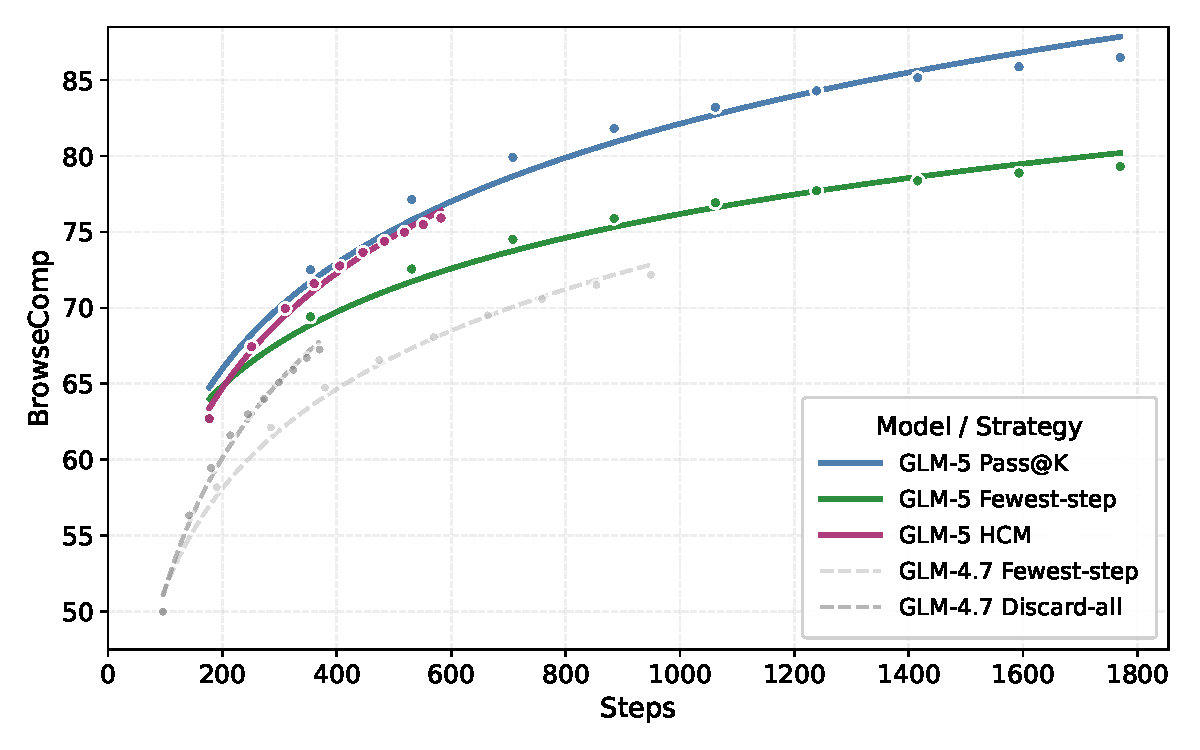
\includegraphics[width=0.7\linewidth]{figures/GLM5-BC-cm.pdf}
    \caption{Accuracy of BrowseComp with different context management strategies from GLM-4.7 (gray baselines) to GLM-5 (colored strategies). }
    \label{fig:GLM5-BC-CM}
\end{figure}







% \section{Advancing Agentic Quality: The MobileRL Framework}
% \todo{check later}

% To further enhance GLM-5’s capabilities in complex, multi-step environments, we integrate the principles of MobileRL, a framework specifically designed to overcome the challenges of online reinforcement learning (RL) for autonomous agents. While Slime provides the infrastructure for scalability, MobileRL introduces the algorithmic refinements necessary to handle the heavy-tailed task difficulty and sparse rewards inherent in real-world agentic tasks.

% \subsection{ADAGRPO: Difficulty-Adaptive Policy Optimization}
% The core of MobileRL is Difficulty-ADAptive Group Relative Policy Optimization (ADAGRPO). Built upon the GRPO foundation used in GLM-4.5, ADAGRPO introduces three strategic enhancements to stabilize training and improve sample efficiency:

% Difficulty-Adaptive Positive Replay (AdaPR): Mobile environments often suffer from sparse terminal rewards, where successful trajectories for difficult tasks are rare but highly informative. AdaPR maintains a curated buffer of these high-quality, challenging trajectories and balances them with on-policy samples to amplify the learning signal and stabilize policy updates.

% Failure Curriculum Filtering (FCF): To prevent the model from wasting computational budget on persistently unsolvable "dead-end" tasks, FCF uses online statistics to down-weight extremely difficult instances. This curriculum-based approach reallocates resources toward feasible but challenging tasks, significantly improving overall sample efficiency.
% x
% Shortest-Path Reward Adjustment (SPA): In multi-turn agentic tasks, standard rewards often fail to penalize verbosity. SPA reshapes the reward function by assigning higher returns to shorter, more efficient solutions. This aligns the model’s behavior with user preferences for speed and efficiency, particularly in real-world coding and GUI navigation.


% \subsection{Two-Stage Reasoning Warm-up}
% Before initiating online RL, MobileRL employs a two-stage Supervised Fine-Tuning (SFT) process to ensure a robust policy initialization:

% Reasoning-Free SFT: Builds a strong foundational action space from expert demonstrations.

% Reasoning SFT: Adds intermediate reasoning traces to improve instruction following, multi-step coordination, and policy transparency.

% \subsection{Empirical Results and State-of-the-Art Performance}
% Integrating MobileRL’s ADAGRPO into the GLM series (e.g., MobileRL-9B based on GLM-4V) has yielded significant performance leaps across major benchmarks.

% Table 2: Success Rates on Mobile Agentic Benchmarks  | Model | AndroidWorld | AndroidLab | | :--- | :--- | :--- | | GPT-4o (2024-11) | 34.5% | 31.2% | | UI-Tars-1.5 (355B) | 64.2% | 38.3% | | MobileRL-9B (Ours) | 80.2% | 53.6% |

% The application of ADAGRPO consistently improves performance across all task complexity levels, with the most substantial relative gains observed in high-complexity tasks (Complexity Level 3+). Furthermore, the introduction of SPA has been shown to consistently reduce the number of steps required for task completion, confirming its effectiveness in optimizing for agentic efficiency.

\subsubsection{Slide Generation}

We employ a self-improving pipeline that aims to systematically enhance slide generation performance by training a specialized slide-generation expert through reinforcement learning and rejection sampling fine-tuning. We first initialize the model with supervised fine-tuning (SFT) to provide a basic slide generation capability, and then perform reinforcement learning with a multi-level reward formulation grounded in common aesthetic and structural properties of presentation slides. This stage leads to substantial improvements in generation quality. We further conduct rejection sampling fine-tuning and mask fine-tuning, allowing knowledge acquired during reinforcement learning to be injected back into the training corpus. This procedure jointly enhances data quality and model capability in a coordinated and iterative manner.

We propose a \textbf{multi-level reward formulation}, which partitions reward signals in the HTML-based slide generation process into three levels:

\textbf{Level-1: Static markup attributes.} This level focuses on declarative attributes in the generated HTML, including positioning, spacing, color, typography, saturation, and other stylistic attributes. Grounded in professional design principles, we design a set of rules to regulate the model’s behavior when generating such declarations. These rules ensure syntactic parsability of the generated HTML, while constraining the design space at the markup level to a subspace optimized for expressiveness, structural clarity, visual harmony, and readability. Additionally, we introduce hallucinated-image and duplicate-image detection mechanisms to suppress hallucinatory or redundant figures.

\textbf{Level-2: Runtime rendering properties.} Unlike static inspection, this level evaluates runtime properties of DOM nodes during rendering, such as element width and height, bounding boxes, and other geometric layout metrics. By constraining these properties, we encourage the generated slides to align more closely with human aesthetic preferences in spatial organization. We develop a distributed rendering service capable of executing rendering jobs at high throughput while extracting the required runtime properties. During training, we observe several forms of reward hacking behaviors, such as hard truncation of overlong content or excessive manipulation of spacing (see Figure~\ref{fig:reward_hacking}). To mitigate these issues, we refine the renderer implementation to eliminate exploitable loopholes, ensuring that reward signals genuinely incentivize aesthetically coherent layouts rather than superficial compliance with geometric metrics.

\begin{figure*}[!thp]
    \centering % 将图居中
    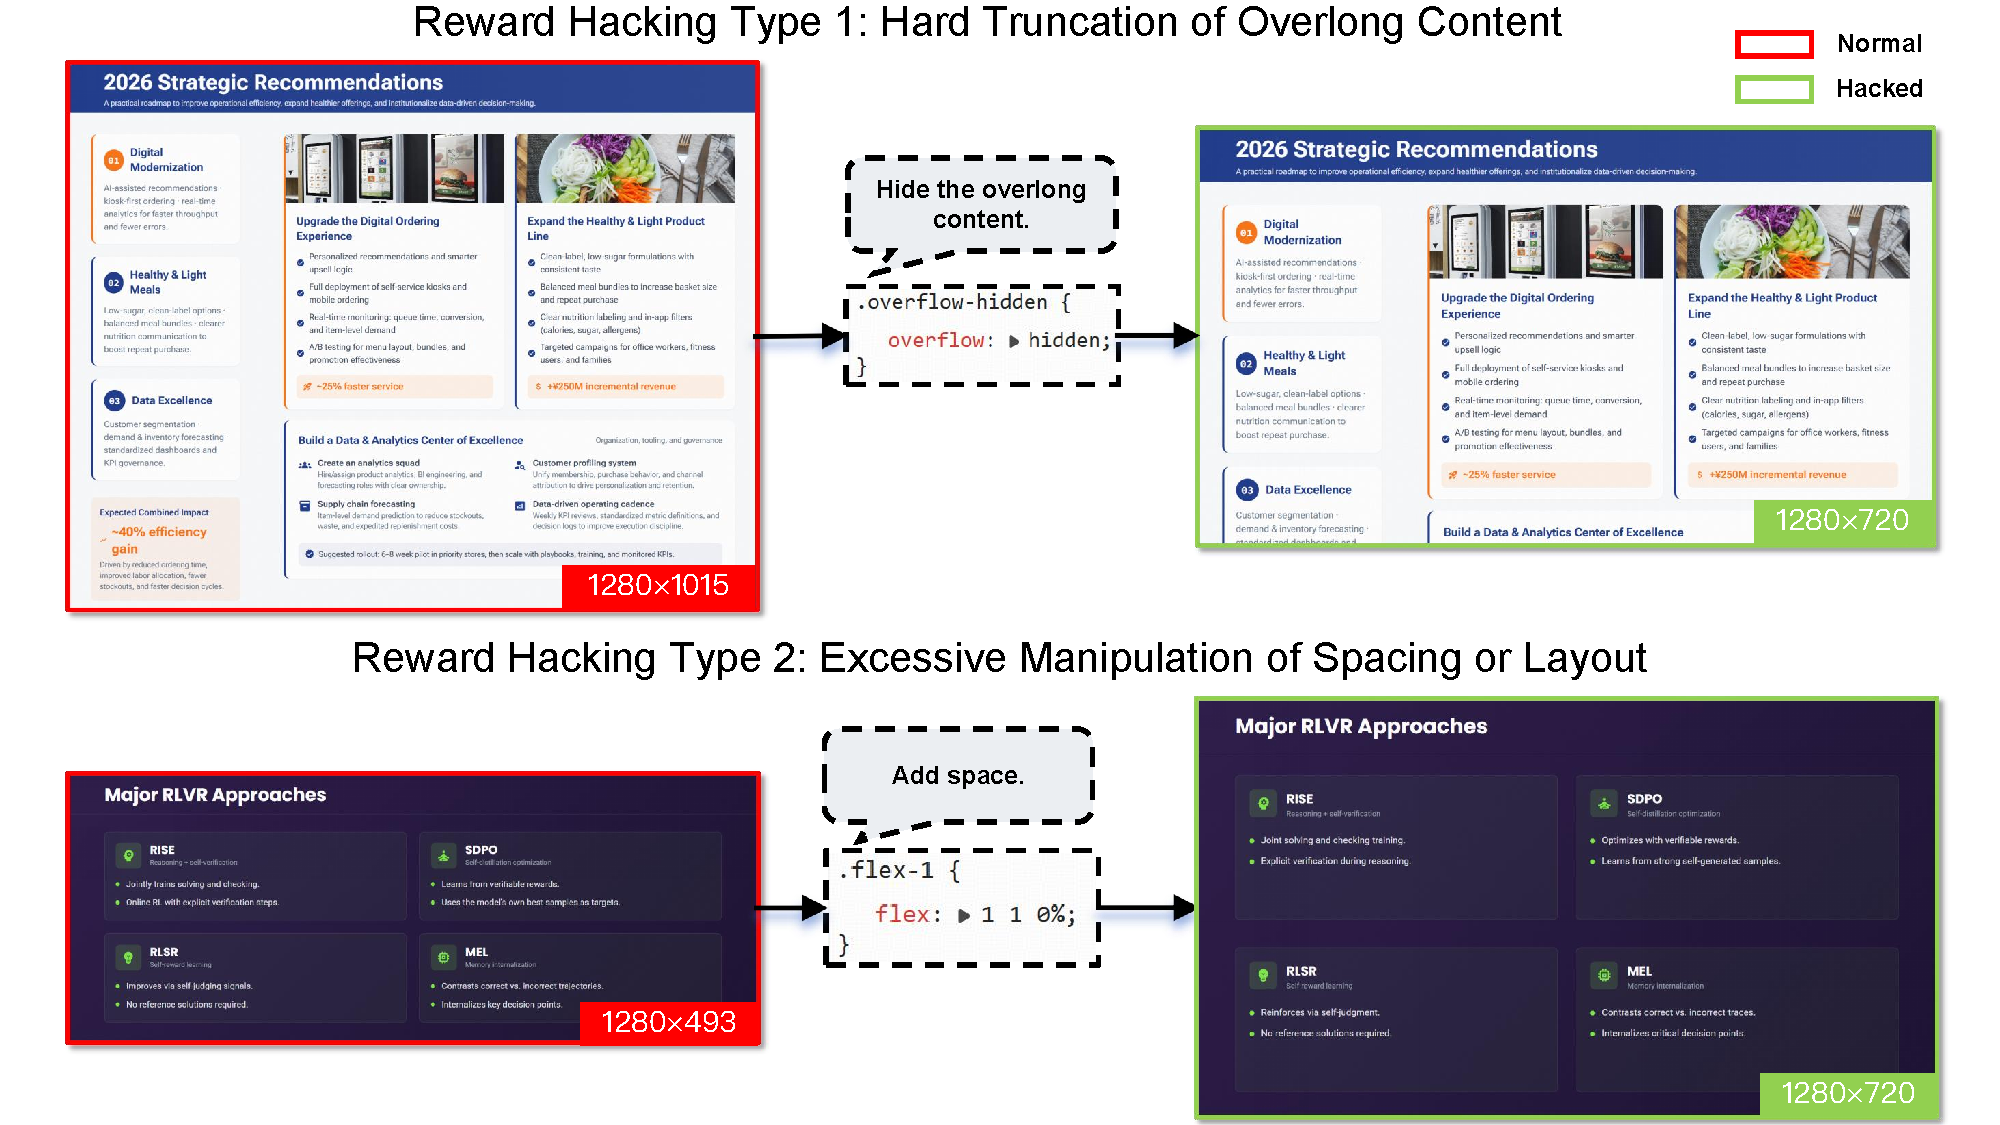
\includegraphics[width=\linewidth]{figures/ppt_reward_hacking.pdf}
   \vspace{-0.1cm}
    \caption{
    Examples of reward hacking in the slides RL training. Our runtime rendering obtains grounded attribute values, making the evaluation robust to such hacking behaviors.
    }
    \label{fig:reward_hacking}
    \vspace{-0.2cm}
\end{figure*}

\textbf{Level-3: Visual perceptual features.} Beyond runtime rendering constraints, we incorporate perceptual-level evaluations of the rendered slides. For instance, we detect abnormal whitespace patterns as an auxiliary signal to further improve overall compositional balance and visual aesthetics.

\textbf{Training strategy.} These signals are jointly optimized during RL to improve the structural validity of generated HTML, enhance layout organization, and elevate overall visual aesthetic quality. In addition to reward design, we reshape the training distribution via dynamic sampling. Specifically, a fraction of structurally trivial samples is probabilistically dropped, allowing optimization to focus on more challenging pages and improving robustness under complex composition scenarios. We also employ a token-level policy gradient loss to stabilize optimization~\cite{yu2025dapo}. Furthermore, we introduce a balancing strategy that distributes different rollout outcomes of the same sample across multiple training batches, reducing optimization bias and improving training stability.


\paragraph{Rejection sampling.}
During the rejection sampling phase, the reward functions used in RL are transferred into a data filtering pipeline to construct a high-quality training subset.
At the page level, filtering criteria include code validity and compilation feasibility. At the trajectory level, we further enforce tool execution correctness and global content diversity constraints, ensuring structural consistency.
We adopt a Best-of-$N$ selection strategy, in which the highest-quality sample is retained from multiple independently generated candidates. This mechanism effectively reweights the distribution toward higher-quality instances, leading to improved sample efficiency and enhanced training stability.

\paragraph{Masking-based refinement.} 
Although rejection sampling removes the majority of low-quality outputs, some trajectories contain defects confined to only a small number of pages. Discarding such samples would reduce effective data utilization and increase generation cost. To address this, we introduce a masking-based correction mechanism that automatically identifies defective pages and applies masking, while retaining the high-quality content within the same trajectory. This selective refinement preserves valuable supervision signals, improves effective data efficiency, and reduces redundant regeneration overhead, thereby enhancing overall training efficiency.

\paragraph{Empirical improvements.}
The proportion of generated pages that strictly comply with the 16:9 aspect ratio increases from 40\% to 92\%, accompanied by a substantial reduction in page overflow cases. Human evaluation further shows that, compared to GLM-4.5, GLM-5 achieves win rates of 60\% in content quality, 57.5\% in layout rationality, and 65\% in visual aesthetics, resulting in an overall win rate of 67.5\%. These results provide empirical evidence for the effectiveness of the proposed multi-level reward design and self-improving framework.

